\section{Evaluation and case studies}
\label{sec:eval}

\paragraph*{Implementation.}
\enumo is an embedded DSL,
  implemented as a \rust library.
The entire implementation
  is 3095 LOC, including unit tests but excluding
  the implementations of the various domains.
The domains together add another 4430 LOC,
 which comprises a grammar, evaluator, and validator for
 each basic domain,
 and a grammar and fast-forwarding rules for
 each domain employing fast-forwarding.
The various \enumo programs add up to 718 LOC.
Our \enumo implementation, the domain implementations, and all the \enumo programs
  are publicly available.

To evaluate our contributions,
  this section answers the following
  research questions.

\begin{enumerate}

\item How does guided enumeration in \enumo
  compare to prior work on rewrite rule synthesis?
  (\autoref{subsec:eval-enumo})

\item Can \enumo scale to larger grammars than
  existing tools can handle?
  (\autoref{subsec:eval-enumo})

\item Can \enumo's fast-forwarding algorithm enable rule
  inference for new domains that prior work could not support?
  (\autoref{subsec:eval-ff})

\item How does fast-forwarding impact client applications
    in terms of performance and results?
    (\autoref{subsec:eval-ff})

\item Can \enumo be extended with new synthesis techniques,
    and do the new operators compose with existing ones?
    (\autoref{sec:case-study-llm})
\item Do the abstractions in \enumo
    enable cross-domain rule synthesis?
    (\autoref{sec:case-study-bv})

\end{enumerate}

\subsection{Guided search with \enumo}
\label{subsec:eval-enumo}

To evaluate \enumo's guided search,
  we conducted the following experiments on a
  64-bit Linux machine with 32 GB RAM,
  running Ubuntu 22.04.2 LTS.

\begin{table}[h]
\resizebox{\textwidth}{!}{%
\begin{tabular}{lcllcc}
Domain   & \enumo LOC  & \# \enumo (Time)   & \# \ruler (Time)  & \enumo $\rightarrow$ \ruler (Time) & \ruler $\rightarrow$ \enumo (Time)  \\ \cline{1-6}
bool & 41 & 64 (0.35)   & 51 (0.05) & 100\% (0.01), 100\% (0.01) & 87.5\% (5.29), 96.9\% (0.01) \\
bv4  & 19 & 180 (7.13)  & 84 (0.96) & 100\% (0.17), 100\% (0.03) & 38.3\% (3.67), 41.1\% (4.32) \\
bv32 & 18 & 120 (48.78) & 78 (13.1) & 100\% (0.15), 100\% (0.01)  & 58.3\% (1.41), 60.0\% (2.08) \\
rational & 57 & 123 (6.34) & 113 (97.9) & 97.3\% (0.73), 100\% (0.09) & 52.0\% (18.66), 58.5\% (22.24) \\
\end{tabular}%
}
\caption{Results comparing \enumo to \ruler.
  $ R_1 ~ \rightarrow ~ R_2$ indicates using $R_1$ to derive
  $R_2$ rules.
  We report both \lhs and \lhsandrhs derivability (in that order), separated by commas.
  The numbers in parentheses are times in seconds.
}
\label{table:oopsla}
\end{table}

\subsubsection{Comparing rulesets with prior work}
\label{subsubsec:e-vs-r}
\ruler~\citep{ruler} is a state-of-the-art
  tool for automatically
  synthesizing rewrite rules targeted towards \eqsat-driven
  systems.
We compare the rules generated by \enumo
  against those generated by \ruler\footnote{bool, bv4, and bv32
  rules are taken from the \ruler artifact. The artifact did not contain
  rational rules, so those were generated following the instructions in
  the \ruler repository on GitHub.},
  finding that
  rulesets from small \enumo programs outperform
  those from \ruler,
  which uses a hard-coded rule-finding
  strategy.
We wrote \enumo programs for
  each of the domains showcased in \ruler:
  \texttt{bool}, \texttt{bv4}, \texttt{bv32}, and \texttt{rational}.
These programs call \T{recursive_rules},
an \enumo-provided utility function (\autoref{fig:rec-rules}).
From a user-provided grammar $\mathcal{G}$ that specifies literal terms,
  unary operators, and binary operators, \T{recursive_rules} builds
  workloads of increasing size, then finds and validates rules from
  the workloads, using rules it finds along the way to avoid redundancy
  in the final ruleset.
This algorithm
 replicates \ruler's core loop in just a few lines of
\enumo code, and could easily be written by an \enumo user,
highlighting the flexibility and power of the tool.
\begin{figure}
\begin{lstlisting}
lang = { LIT (UOP EXPR) (BOP EXPR EXPR) }
def recursive_rules($\mathcal{G}$, metric, n):
  if n == 0: return []
  rec_rules = recursive_rules($\mathcal{G}$, metric, n - 1)
  workload = iter_metric(lang, "EXPR", metric, n)
               .plug("LIT", $\mathcal{G}$.lits).plug("UOP", $\mathcal{G}$.uops).plug("BOP", $\mathcal{G}$.bops)
  rules_n = workload
              .to_egraph()
              .compress(rec_rules)
              .find_candidates()
              .minimize(rec_rules)
  return rec_rules.union(rules_n)
\end{lstlisting}
\caption{The \T{recursive_rules} function. $\mathcal{G}$ is a struct that
  specifies a grammar, containing workloads for literal expressions,
  unary operators, and binary operators. \T{metric} is the \enumo metric
  used to define an upper bound on terms, and \T{n} is the size limit.
  \T{recursive_rules} incrementally builds a ruleset by learning rules
  over terms from the domain of increasing size up to the
  specified limit.}
\label{fig:rec-rules}
\end{figure}

After running our \enumo programs,
we compared the derivability of the generated rulesets
to those produced by \ruler,
using the same grammar and interpreter.
We found that for rational arithmetic,
  \ruler learns rules over division by assuming that
  the denominator is not zero\footnote{To mitigate the resulting
  unsoundness, \ruler used a custom rule application
  strategy from the \egg~\citep{egg} library.}.
We removed this unsound
  assumption from \ruler and re-synthesized its
  rational arithmetic rules for our comparison.
We also found that for \C{bool}, \C{bv4}, and \C{bv32}, \ruler's hard-coded
  term enumeration loop does not enumerate any constant values.
As a result, \ruler fails to learn simple identities like \C{(\& ?a (~ ?a)) \rewritesto \, false}
  and \C{(<< ?a 0) \rewritesboth \, ?a}.
Failure to enumerate these constants explains why \ruler is unable to derive
  many of \enumo's rules for these domains.
We adapted the \enumo programs to not enumerate constants, and we find that
  \ruler can derive 100\% of the \C{bool} rules, 90.7\% of the \C{bv4} rules,
  and 87.8\% of the \C{bv32} rules\footnote{Both \lhs and \lhsandrhs derivability
  result in these percentages.}.

We found that \enumo rulesets were able to derive
  all of \ruler's rules using \ruler's
  own \lhsandrhs derivability metric
  (\autoref{subsec:derivability}, \autoref{table:oopsla}).
The reverse is not true.
Using the more conservative \lhs metric, \enumo rulesets derive
  a higher percentage of \ruler's rules than \ruler's rules can derive of
  \enumo's.
Both measures suggest that \enumo rulesets have greater proving power
  than their \ruler counterparts.
This result demonstrates that small (\C{<}60 LOC), simple
\enumo programs outperform \ruler while also providing users
with increased flexibility and transparency.

\subsubsection{Scaling to large grammars: A Halide case study}
\label{subsec:halideeval}
Halide~\citep{halide} is a programming language
  for high-performance
  image processing.
A major component of the Halide compiler is
  a traditional term rewriting
  system~\citep{julie-halide} that performs optimizing
  program transformations using a set of handwritten rules.
Halide has a large grammar, totaling 17 operators,
  which include boolean,
  arithmetic, and
  comparison operators.
Halide does not use an \eqsat engine
  for applying the rewrite rules.
Nevertheless, inspired by the domain,
  particularly due to the size of its grammar,
  we developed an \enumo program to evaluate
  the scalability of \enumo's workload-guided strategy.

Halide's handwritten ruleset was collected by scraping
source files from the latest commit in the Halide
  repository\footnote{\url{https://github.com/halide/Halide/commit/e7f78600e10956b44e8f214c686f310211b0d836}}
  and removing rules that we could not parse as \enumo rules.
These included rules with side conditions, rules with unsupported operators,
  and rules with unbound variables on the right-hand side of the rule.
After this process, we were left with 725 rules.

To see how prior work~\citep{ruler}
  would perform on a large domain,
  we implemented the Halide grammar in \ruler. \ruler's
  implementation was able to run for
  just one iteration (further iterations did not terminate),
  synthesizing a total of 90 rules in about 3 seconds.
  This ruleset was able to derive
  only 18 of the 725 original rules (2.5\%)
   using both derivability metrics (\lhs, \lhsandrhs).

Without leveraging guided search, \enumo scales similarly to Ruler
  for exhaustive exponential searches.
A simple \enumo program that exhaustively enumerates Halide terms up to size
  5 is able to derive 327 of Halide's 725 rules.
The exhaustive \enumo program only outperforms \ruler because \ruler
  enumerates by depth, which grows much faster than size.
An \enumo program that enumerates by depth times out after depth 2 and learns
  rules that can only derive 13 of Halide's rules, which is similar to
  \ruler's behavior.

However, the key benefit of \enumo's guided enumeration is decoupling
  the grammar and the workload size.
In \ruler, terms are enumerated exhaustively from the grammar up to a
  certain size, so with a larger grammar, \ruler hits resource limits
  faster.
In contrast, term enumeration in \enumo is separate from the
  grammar itself, allowing users to define workloads that represent
  different subsets of the search space.
With \enumo's operators, it is easy to compose workloads together,
  enabling a piecewise rather than total approach to term enumeration.
This composability makes it possible to synthesize rulesets that are
  larger and deeper than would be possible with a one-shot theory
  exploration tool like \ruler.

To evaluate whether \enumo's
  guided search would help to find deeper, more complex Halide rules,
  we wrote a 141-line \enumo program
  leveraging both exhaustive and custom enumeration.
  First, we exhaustively enumerated terms over subsets of Halide's
  operators---boolean, arithmetic,
  comparison\footnote{For both \ruler and \enumo,
  we enumerated terms over
  15 of the 17 operators, skipping $/$ and $\implies$ since
  most of those rules had side conditions.}%
  ---up to 5 atoms, beyond which point this strategy
  is computationally infeasible.
  We then enumerated
  terms with \textit{all} of
  Halide's operators up to
  4 atoms in size.
Finally, we created custom
  workloads guided by domain knowledge,
  selectively generating terms too large to be
  found using the exhaustive approach,
  such as \C{(select a (min b c) (max d c))}.
  These workloads leverage \enumo features
  such as canonicalization
  (\autoref{sec:slide}), which eliminates many duplicate terms,
  reducing one workload
  from 52,491 to 9,233 terms---an 82\%
  decrease\footnote{More details on how the Halide programs
  were written are available in \autoref{subsec:halide-appendix}.}.
 Ultimately, our \enumo program produced a ruleset of 840 rules
  capable of deriving
  84.0\% and 90.9\% of the handwritten ruleset using
  the \lhs and \lhsandrhs derivability
  metrics, respectively.

As mentioned in \autoref{subsec:derivability}, larger rulesets are not
  necessarily better than smaller rulesets.
In this case study, however, the smaller ruleset (from one iteration of \ruler)
  has measurably less proving power than the larger ruleset
  (from the \enumo program), so the additional rules are justified.
Synthesizing rulesets for large grammars is not feasible
  with tools that rely on exhaustive term enumeration,
  but with \enumo, it is possible to build
  rulesets incrementally, so grammar size is not a
  limiting factor.
This section shows that a small program
using \enumo's novel guided search finds better rules than
the state of the art can.


\subsection{Fast-forwarding}
\label{subsec:eval-ff}

In this section,
  we evaluate our new \ff algorithm (\autoref{sec:lift})
  in two new domains to learn rewrite rules
  that other state-of-the-art tools
  do not support.
We also show that synthesized rules from \enumo
  can be easily integrated with
  existing \eqsat-based synthesis tools.

\begin{table}[h]
\resizebox{\textwidth}{!}{%
\begin{tabular}{lllccc}
Domain      & \enumo LOC  & \# \enumo (Time)  & \# \herbie  & \enumo $\rightarrow$ \herbie (Time) & \herbie $\rightarrow$ \enumo (Time)  \\ \cline{1-6}
  Exponential &  186  & 40 (3.58)    & 82 &  39.0\% (1.03), 43.9\% (1.25)   & 100\% (0.24), 100\% (0.01) \\
  Rational    &   82  & 129 (276.16) & 87 &  70.1\% (54.77), 73.6\% (55.19) &  -, -\\
  Trigonometric  &  160  & 56 (631.94)  & 45 &  33.3\% (4.20), 35.6\% (7.36) & 46.4\% (0.84), 46.4\% (2.27)\\
\end{tabular}%
}
  \caption{
  Derivability comparison between rules from \enumo and \herbie.
  As in \autoref{table:oopsla},
    $R_1 ~ \rightarrow ~ R_2$ indicates using
    $R_1$ to derive $R_2$ rules.
  For Exponential and Trigonometric, we include the trusted arithmetic
    rules defined below (\C{RAT}, and \C{R} without its division
    rules) when computing the derivability.
  We report both \lhs and \lhsandrhs derivability
    (in that order), separated by commas. The numbers in parentheses
    are times in seconds.
 ``-'' indicates that the derivability test
    could not be completed due to \herbie's
    unsound rules (\autoref{para:herbie}).
  We integrate these rules for
    end-to-end runs of \herbie~\citep{herbie} and
    Megalibm~\citep{megalibm} (\autoref{subsubsec:numbers}).}
\label{table:herbie}
\end{table}

\subsubsection{Numeric domain}
\label{subsubsec:numbers}

We used the fast-forwarding algorithm together with
  guided enumeration to infer rewrite rules
  for the domain of transcendental functions.
To evaluate the quality of the rulesets,
  we integrated the rules into two existing
  rewrite-rule-based synthesis tools,
  \herbie~\citep{herbie} and
  Megalibm~\citep{megalibm}.

\paragraph*{Trigonometric and exponential representation.}
\label{eval:trig-rep}

Recall that sine and cosine have representations
  in terms of the complex exponential $\cis(x)$
  (\autoref{subsec:ffoverview}).
The trusted rules for the Trigonometric domain fall into three groups, which we refer
  to throughout the evaluation:
\begin{itemize}
  \item \C{R}: 57 automatically generated arithmetic rules,
    including 13 rules involving division that are sound only when their divisors are nonzero\footnote{
      In our \enumo programs for this domain, we are careful to exclude undefined terms from the \egraph,
      so the potentially unsound rules are harmless. Herbie uses unsound rules in its \eqsat
      runs, but with extra checks to detect unsound merges and recover from them.
    }.
  \item \C{C}: 15 handwritten rules about the complex exponential, including rules like
  $\cis(a + b) \leftrightsquigarrow \cis(a) \cdot \cis(b)$,
  $\cis(0) \leftrightsquigarrow 1$, and $i \cdot i \leftrightsquigarrow -1$.
  \item \C{E}: 18 \textit{exploratory} rules (\autoref{sec:lift}), which
    give the definitions of $\sin$, $\cos$, and $\tan$ in terms of $\cis$, $i$, and $\pi$.
\end{itemize}

Similarly, the logarithmic, power, square root,
  and cube root functions are all defined in terms of $e^x$,
  the real exponential function:
  $e^{\log(x)} \leftrightsquigarrow x$,
  $a^b \leftrightsquigarrow e^{b \cdot \log(a)}$,
  $\sqrt{a} \leftrightsquigarrow e^{1/2 \cdot \log(a)}$, and
  $\sqrt[3]{a} \leftrightsquigarrow e^{1/3 \cdot \log(a)}$.
In the exponential domain, we have two trusted rulesets:
\begin{itemize}
  \item \C{RAT}: 141 automatically generated arithmetic rules
  \item \C{EXP}: 13 handwritten rules involving the real exponential function,
    which include rules that define
    $\log$, powers, and roots in terms of $e^x$,
  to bootstrap fast-forwarding.
\end{itemize}
For both the exponential and trigonometric domains,
  the set of known arithmetic rules can be produced by
  \enumo~via methods described in previous sections.

\paragraph*{\herbie.}

\herbie~\citep{herbie} is a widely used, open-source tool
  for improving the accuracy of floating-point expressions.
Given a mathematical expression over real numbers,
  it synthesizes a more accurate
  floating-point implementation
  using a variety of techniques
  including equality saturation.
\herbie's equality saturation-based optimization pass
  uses a set of 358 expert-written rewrite rules
  to explore many programs
  that are equivalent over the reals,
  keeping only those that have
  lower floating-point error.
\herbie's rewrite rules include many algebraic identities
  about rational arithmetic, trigonometry, and exponents.

\paragraph*{Results.}
\label{para:herbie}
\begin{figure}
  \begin{subfigure}[t]{0.49\linewidth}
    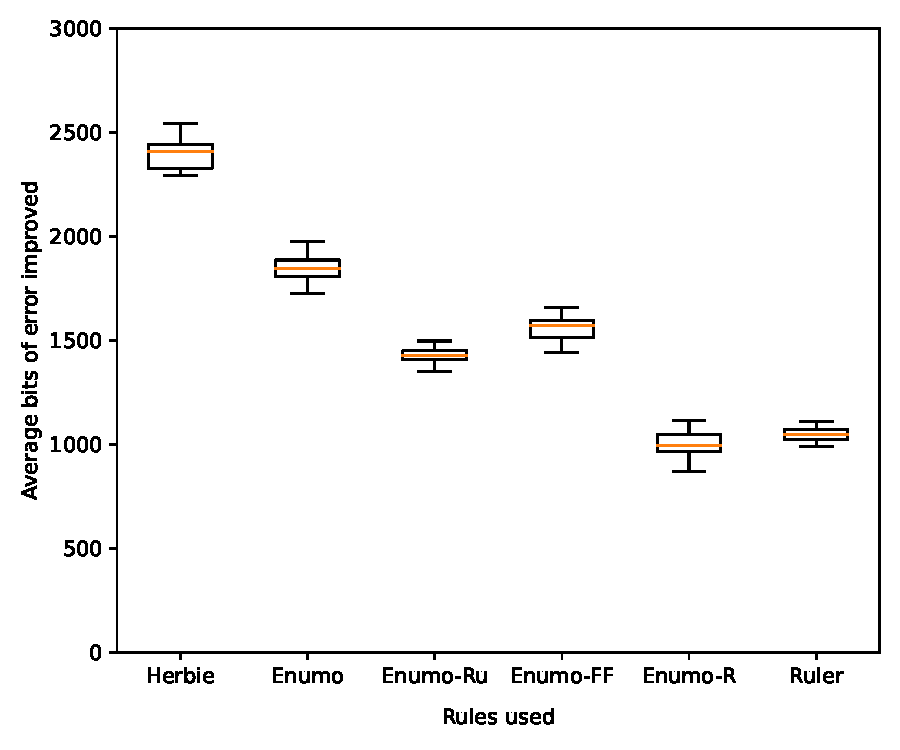
\includegraphics[width=\linewidth]{fig/herbie/err-improve.pdf}
  \end{subfigure}
  \hfill
  \begin{subfigure}[t]{0.49\linewidth}
    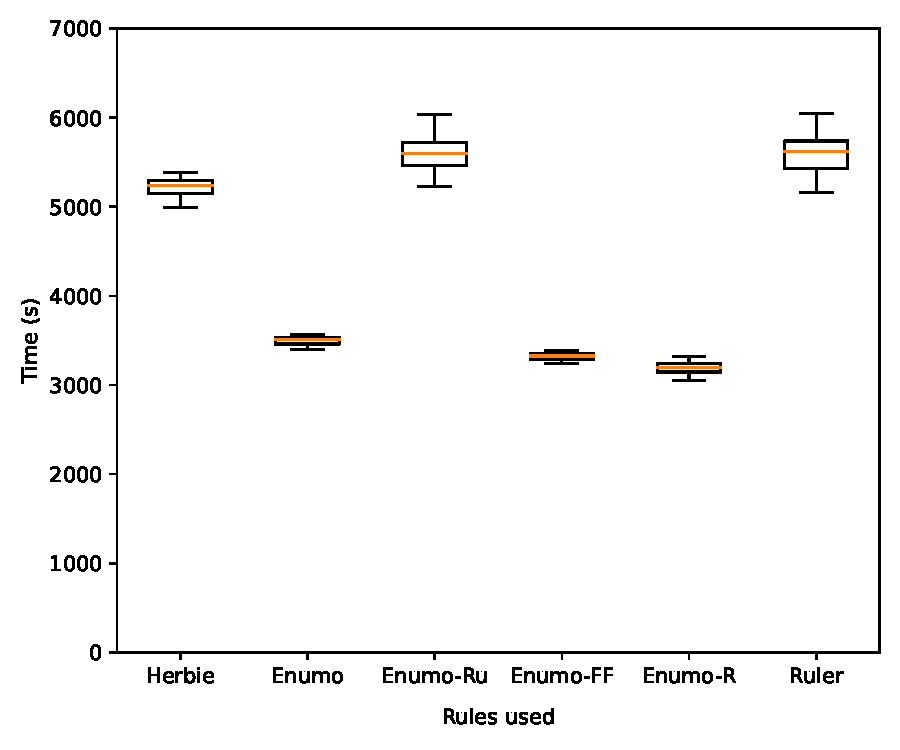
\includegraphics[width=\linewidth]{fig/herbie/time.pdf}
  \end{subfigure}
  \caption{
    Comparison of different rules on \herbie's
      end-to-end performance for six different configurations:
      \herbie's default rules (\texttt{Herbie}),
      \enumo's rules (\texttt{\enumo}),
      \enumo's rules with its rational rules replaced by \ruler's rational rules (\texttt{\enumo-Ru}),
      \enumo's rules without fast-forwarded rules (\texttt{\enumo-FF}),
      \enumo's rational rules (\texttt{\enumo-R}),
      and \ruler's rules (\texttt{\ruler}).
    The two plots show
      (left) \herbie's metric for measuring accuracy (higher is better); and
      (right) \herbie's running time (lower is better).
    Each boxplot represents the results from 30 seeds,
     where each data point is obtained by summing the values
     (average error, time) over the 170 benchmarks that
     finish within the time limit.
    \enumo's rules allow \herbie to improve error
      significantly more than \ruler's rules.
  }%
  \label{fig:herbie-res}
\end{figure}

First, we wrote \enumo programs to synthesize boolean,
  rational, trigonometric (fast-forwarded),
  and exponential (fast-forwarded) rules for \herbie.
The summary of these results is in \autoref{table:herbie}.
Note that \enumo's rules derive only about a third of
  \herbie's trigonometric ruleset:
  \herbie's handwritten rules include forms beyond
  the scope of our workloads and, as discussed below,
  some unsound rules that no sound ruleset can derive.
Then, based on suggestions from \herbie's developers,
  we filtered the \herbie benchmark suite to 176
  representative benchmarks, taken from a variety of domains,
  including graphics, mathematics, and numerical analysis.
In addition, we disabled polynomial approximation to
  isolate the effects of \eqsat within \herbie.
We ran \herbie on the benchmarks under six different configurations:
\begin{itemize}
  \item \foottt{\herbie}: \herbie's default configuration.
  \item \foottt{\enumo}: \enumo's rules, including boolean, rational, trigonometric, and exponential.
  \item \foottt{\enumo-Ru}: \enumo's rules with its rational rules replaced by \ruler's rational rules. This includes \enumo's boolean, trigonometric, and exponential rules, and also \ruler's rational rules.
  \item \foottt{\enumo-FF}: \enumo's rules without fast-forwarded rules.
  \item \foottt{\enumo-R}: \enumo's rules, including only
  boolean and rational rules.
  \item \foottt{Ruler}: We compare against \ruler's rules~\citep{ruler}
    for the rational and boolean domains.
    \ruler does not support the trigonometric and exponential domains.
\end{itemize}

We used the default node limit of 8000 nodes
  in \herbie's underlying \eqsat engine,
  i.e., upon hitting the limit,
  the engine stops applying the simplification rules.
On 6 benchmarks, \herbie does not finish
  within 300 seconds; we discard these.
For all six configurations,
  we ran \herbie on 30 seeds.

\autoref{fig:herbie-res} shows the results of running
  \herbie with one boxplot for each ruleset configuration.
The left plot
  shows the improvement in accuracy achieved by \herbie,
  measured in \herbie's ``bits of error'' metric:
  the number of ``incorrect'' bits
  in the binary representation of the floating-point
  result against a high-precision oracle
  (higher improvement is better).
The right plot shows the average running time of \herbie;
  \enumo's rules consistently yield faster runs
  than \ruler's rules.
\herbie's handwritten ruleset (\herbie) finds the
  most accurate programs, followed by \enumo's rules.
This experiment offers two key takeaways:
  (1) \ff is valuable in practice, and (2) \ff and
  guided search combined lead to better rulesets than
  exhaustive synthesis alone.

Disabling trigonometric and exponential rules (\texttt{\enumo-FF}),
  \emph{but leaving the rules needed to bootstrap fast-forwarding},
  results in a significant drop in accuracy,
  demonstrating that fast-forwarding is necessary in
  the face of resource limits.
By definition, the rulesets from both \texttt{\enumo} and \texttt{\enumo-FF} have equal proving power,
  but \autoref{fig:herbie-res} demonstrates
  a significant advantage for \texttt{\enumo} over \texttt{\enumo-FF} in practice.
Using only the rational rules (\texttt{\enumo-R}) also results in lower accuracy,
  showing that trigonometric and exponential rewrite rules are important for \herbie.

To our surprise,
  Ruler's rational rules (\texttt{\ruler}) outperformed
  those from \enumo (\texttt{\enumo-R}).
However, we show that when combined with the rest of
  \enumo's ruleset (\texttt{\enumo}), \enumo finds more accurate programs
  faster than \ruler.
Replacing \enumo's rational rules with \ruler's (\texttt{\enumo-Ru})
  results in a significantly worse ruleset.
The reason is that the combination of \enumo's rational ruleset
  and \enumo's trigonometric and exponential rules allows \herbie
  to fix a wider range of floating-point errors.
We suspect that \enumo's rational rules (\texttt{\enumo-R}) explore a larger
  space than \ruler's (causing \herbie to exceed resource limits faster)
  without any benefit, leading to a slight accuracy loss compared to
  \ruler's rational rules.

An example of where rules from \enumo excel over rules from \ruler
  is \herbie's ``2cos''%
  \footnote{\url{https://github.com/herbie-fp/herbie/blob/d35c6a3cc7ab/bench/hamming/trigonometry.fpcore}}
  benchmark, $\cos(x + \varepsilon) - \cos x$,
  which suffers from error when $\varepsilon$ is relatively small.
With \enumo's ruleset,
  \herbie~uses the essential rewrite
  \C{(cos (+ b a)) \rewritesto ~} \\
  \C{(- (* (cos b) (cos a)) (* (sin b) (sin a)))}
  to decompose $\cos(x + \varepsilon)$, and then
  eliminates cancellation using associative rules.
The full rewrite is
  $\cos(x + \varepsilon) - \cos x
  \rightsquigarrow
  \cos x \cdot (\cos\varepsilon + -1) + \sin x \cdot (-\sin\varepsilon)$.

However, \herbie still finds more accurate programs
  with its handwritten ruleset.
One significant reason for this difference is that
  \herbie often relies on unsound
  division, trigonometry, and exponentiation rules in order
  to eliminate sources of errors
  such as cancellation without checking if
  such transformations are correct for all arguments.
For example,
  for the benchmark ``2sin''%
  \footnote{\url{https://github.com/herbie-fp/herbie/blob/d35c6a3cc7ab/bench/hamming/trigonometry.fpcore}},
 \herbie rewrites
 $\sin \left(x + \varepsilon\right) - \sin x$ to
 $\cos x \cdot \sin \varepsilon + ({\sin \varepsilon}^{2} \cdot \sin x)/(-1 - \cos \varepsilon)$
 using a series of rewrites including the unsound
 factoring rule
 \C{(+ a b)} \rewritesto ~ \C{(/ (- (* a a) (* b b)) (- a b))},
 which is invalid when \C{a} equals \C{b}.
In contrast, \enumo generates a conditional
  factoring rule with the side condition $(- a b) \neq 0$.
Unfortunately, \herbie is not designed to leverage conditional rules.
With \enumo, however, we can instead reify the guard syntactically
  within the rewrite itself.
\herbie can directly apply such rules, e.g.,
  \C{(+ a b)}
  \rewritesto ~
  \C{(if (- a b)
         (/ (- (* a a) (* b b)) (- a b))
         (+ a b))},
relying on other rules to simplify the condition syntactically.
\herbie's use of unsound rules and its lack of support
  for conditional rules pose a significant challenge in
  closing the gap between its handwritten rules
  and \enumo's generated rules.



\newcommand{\baselineCosImpls}{16~}
\newcommand{\baselineCosUnique}{4~}
\newcommand{\baselineCosUniqueIds}{2~}

\newcommand{\enumoCosImpls}{8~}
\newcommand{\enumoCosUnique}{5~}
\newcommand{\enumoCosUniqueIds}{3~}

\paragraph*{Megalibm.}
Next, we show how the
  ruleset inferred using \enumo for \herbie
  is also useful for
  Megalibm~\citep{megalibm}, another \eqsat
  tool that relies on numeric rewrites.
Given a transcendental operator,
  e.g., $\cos$,
  Megalibm synthesizes a set of low-level implementations
  that make different speed vs.\ accuracy tradeoffs.
A core phase in Megalibm
  is using \eqsat to discover various
  identities over such operators.

Using sound rules from
  rational, trig, and exponential \enumo programs (\autoref{table:herbie}),
  we ran the Megalibm benchmarks for $\sin$, $\cos$, and $\tan$.
Compared to Megalibm's manually developed ruleset,
  \enumo's rules would ideally discover
  at least as many \textit{unique} identities, in turn
  hopefully yielding as many or more \textit{unique}
  implementations across the speed vs.\ accuracy tradeoff space.

We detail the results for $\cos$ where
  the Megalibm baseline found the following identities:
  $\cos(x) = \cos(x + 4\pi)$,
  $\cos(x) = \cos(x + \pi + \pi)$,
  $\cos(x) = 2\cdot2\cdot \cos(-x) ~/~ 4$, and
  $\cos(x) = (\pi+\pi) - ((\pi+\pi) - \cos(-x))$.
The third and fourth identities are equivalent:
  both can be simplified to $\cos(x) = \cos(-x)$.
Similarly, the first identity
  is just two applications of the second.
Thus, the baseline only yielded 2 unique identities,
  from which Megalibm generated
  \baselineCosUnique implementations
  with differing speed and accuracy.
With \enumo-generated rewrite rules,
  Megalibm produces the following identities:
  $\cos(x) = \cos(x + (\pi + \pi))$,
  $\cos(x) = \cos(-x) \cdot 2 / 2$,
  $\cos(x) = \cos(\pi - x) - (\cos(\pi - x) \cdot 2)$,
  $\cos(x) = \cos(\pi - x) \cdot (- (\cos(\pi - x))^0)$, and
  $\cos(x) = -\cos(\pi - x)$.
Here, the third, fourth, and fifth identities are equivalent,
  yielding \enumoCosUniqueIds unique identities,
  which Megalibm used to find \enumoCosUnique unique implementations.
For $\tan$, Megalibm was able to use
  \enumo-generated rules to find
  \textit{new} identities of $\tan$
  where the baseline ruleset did not derive any.

\autoref{fig:megalibm-results} shows
  Megalibm's estimates of the speed vs.\ accuracy
  tradeoffs for implementations of $\cos$ generated by
  the \enumo-generated and manually developed baseline rulesets.
The table summarizes how,
  across $\sin$, $\cos$, and $\tan$,
  rules from \enumo always produced
  more unique identities,
  which typically also led to more unique implementations---except
  $\sin$, where
  the baseline yielded two extra implementations.
\enumo's rulesets
  can be applied across different tools in
  related domains and perform similarly to or better
  than manually developed expert rulesets.

\begin{figure}[t!]
  \centering
  \begin{subfigure}[T]{0.41\linewidth}
  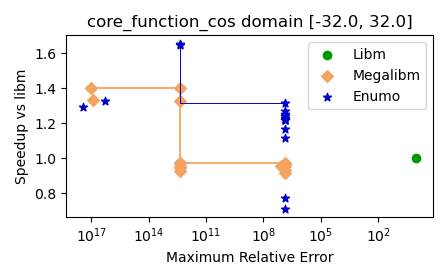
\includegraphics[width=\linewidth]{fig/megalibm/cos-3-pareto.png}
  \label{fig:megalibm-impls}
\end{subfigure}
  \hfill
  \begin{subfigure}[T]{0.58\linewidth}
    \centering
    \vspace{2em}
    \footnotesize
  \begin{tabular}{ccccc}
    \multirow{2}{*}{Fn} & \multicolumn{2}{c}{Megalibm} & \multicolumn{2}{c}{\enumo} \\ \cline{2-5}
    & \multicolumn{1}{c}{Unique Impls} & Unique Ids & \multicolumn{1}{c}{Unique Impls} & Unique Ids \\ \hline
    sin & \multicolumn{1}{c}{7} & 2 & \multicolumn{1}{c}{5} & 3 \\
    cos & \multicolumn{1}{c}{4} & 2 & \multicolumn{1}{c}{5} & 3 \\
    tan & \multicolumn{1}{c}{\color{red}{0}} & \color{red}{0} & \multicolumn{1}{c}{3} & 1  \\
    \end{tabular}
\end{subfigure}
  \caption{Megalibm analysis.
  (Left)
  The Pareto curve shows
    the implementations Megalibm found for
    cosine over the interval [-32.0, 32.0], with
  results normalized to the GNU libm implementations.
  Points up and to the right are better (faster and less error).
  Uniqueness is judged by clusters of performance.
  (Right)
  The number of unique identities and
    implementations generated with Megalibm's original rules
    and \enumo-synthesized rules.
  Notably,
    Megalibm found no identities or implementations for
    $\tan$, but \enumo did.
  }%
  \label{fig:megalibm-results}
\end{figure}


\subsubsection{Geometric domain}
\label{subsec:geo-domain}
\newcommand{\Caddy}{\textit{Caddy}\xspace}
\newcommand{\CoreCaddy}{\textit{Core Caddy}\xspace}

\sz~\citep{szalinski} is an \eqsat-driven
  tool that shrinks 3D CAD (Computer-Aided Design) programs
  by performing rewrites
  over a language called \Caddy.
  \Caddy expresses CAD programs with
  primitives for
  constructive solid geometry (e.g., \C{Cube}, \C{Scale}, \C{Union}),
  basic rational arithmetic,
  various list constructors,
  and inverse transformations.
\sz shrinks \Caddy programs using
  two rulesets:
  a set of CAD
  identities
  and a set of custom procedural rewrite rules
  which discover opportunities to use inverse
  transformations.

We focus on synthesizing
  the CAD identities,
  which help \sz expose
  hidden structure in its input programs.
Synthesizing these identities using
  traditional rule inference algorithms
  requires a full CAD interpreter,
  which is difficult to implement and
  too slow for use in rule synthesis.
Instead, we leverage \enumo's \ff approach.

\paragraph*{Synthesizing CAD identities.}
Solid geometry can be
  represented mathematically via
  a function representation (F-Rep).
An F-Rep is a function $f(x, y, z)$
  which interprets an arithmetic expression
  over $x$, $y$, and $z$ as the geometric solid
  defined where $f$ is positive~\citep{frep}.
For example, the unit sphere can be represented
  by $1 - x^2 - y^2 - z^2$.

We use \enumo to synthesize a set of CAD
  identities by
  fast-forwarding from a small set of 5
  translational rules from CAD to F-Rep
  combined with 15 rules over the F-Rep domain.
Our prior rules for F-Rep included 6 rules
  over rationals and 9 substitution rules
  over operators that allowed it to express \Caddy
  transformations.
Here are two examples of these rules:
\[
  \mathit{Sphere}(r) \rewritesto  1 -  \left(\frac{x}{r}\right)^2 - \left(\frac{y}{r}\right)^2 - \left(\frac{z}{r}\right)^2
  \qquad
  \mathit{Scale}([w, h, l], e) \rewritesto e\left[ x \mapsto \frac{x}{w}\right]\left[ y \mapsto \frac{y}{h}\right]\left[ z \mapsto \frac{z}{l}\right]
\]
Using \enumo's guided search and fast-forwarding,
  we synthesized a set of 10 large bidirectional
  CAD identities of up to 13 atoms:
\begin{enumerate}
  \item \foottt{(Trans (Vec3 0 0 0) a) \rewritesboth \xspace a}
  \item \foottt{(Scale (Vec3 1 1 1) a) \rewritesboth \xspace a}
  \item \foottt{(Cylinder (Vec3 b b b) a true) \rewritesboth \linebreak
    (Scale (Vec3 b b b) (Cylinder (Vec3 1 1 1) a true))}
  \item \foottt{(Sphere b a) \rewritesboth \xspace (Scale (Vec3 b b b) (Sphere 1 a))}
  \item \foottt{(Scale (Vec3 f e d) (Cube (Vec3 c b a) false)) \rewritesboth \linebreak
    (Scale (Vec3 (* f c) (* e b) (* d a)) (Cube (Vec3 1 1 1) false))}
  \item \foottt{(Cube (Vec3 (* f e) (* d c) (* b a)) false) \rewritesboth \linebreak
    (Scale (Vec3 f d b) (Cube (Vec3 e c a) false))}
  \item \foottt{(Trans (Vec3 g f e) (Scale (Vec3 d c b) a)) \rewritesboth \linebreak
    (Scale (Vec3 d c b) (Trans (Vec3 (/ g d) (/ f c) (/ e b)) a))}
  \item \foottt{(Scale (Vec3 g f e) (Trans (Vec3 d c b) a)) \rewritesboth \linebreak
    (Trans (Vec3 (* d g) (* c f) (* b e)) (Scale (Vec3 g f e) a))}
  \item \foottt{(Scale (Vec3 g f e) (Scale (Vec3 d c b) a)) \rewritesboth \linebreak
    (Scale (Vec3 (* g d) (* f c) (* e b)) a)}
  \item \foottt{(Trans (Vec3 (+ g f) (+ e d) (+ c b)) a) \rewritesboth \linebreak
    (Trans (Vec3 g e c) (Trans (Vec3 f d b) a))}
\end{enumerate}

The workload we used is shown in \autoref{fig:szalinski-workload}.

\paragraph*{Results.}
We evaluate \sz's performance
  on a set of
  benchmarks taken from the paper (Table 2 of \citealt{szalinski})\footnote{
    \citet{szalinski} states that
     these benchmarks were decompiled using the
     Reincarnate~\citep{reincarnate} mesh decompiler.}.
The results are shown in \autoref{fig:szalinski-results}.
Using \enumo's synthesized rules for CAD identities, \sz is able
  to shrink input benchmarks by 87\% on average, while the original, handwritten
  rules shrink input benchmarks by 90\% on average.
Upon closer inspection, we found that a subset of the \enumo-synthesized
  rules matches the performance of \sz's handwritten CAD identities.
There are some rules in the \enumo ruleset that
  cannot be derived from \sz's CAD identities.
However, we posit that these additional rules
  are not very useful for the \sz benchmark tests, so their
  presence in the \enumo ruleset leads to worse
  performance at low node limits.

\begin{figure}

  \begin{lstlisting}[
    name=szalinski-workload-code,
    language=Python,
    basicstyle=\footnotesize\ttfamily,
    numbers=left,
    xleftmargin=2.5em]
  def iter_szalinski(n):
    lang = { (AFFINE VEC SOLID) (Cube VEC) (Cylinder VEC) (Sphere SCALAR) }
    return iter_metric(lang, "SOLID", Depth, n)
             .plug("VEC", { (Vec3 0 0 0) (Vec3 1 1 1) (Vec3 a a a) (Vec3 a b c)
                           (Vec3 d e f) (Vec3 (BOP a d) (BOP b e) (BOP c f)) })
             .plug("AFFINE", { Scale Trans })
             .plug("SCALAR", { a 1 })
             .plug("BOP", { + * / })

  cad_idents = []
  for i in [2, 3]:
      wkld = iter_szalinski(i)
      chosen = fast_forward(wkld, frep_rules, cad_idents)
      cad_idents.extend(chosen)
  \end{lstlisting}
  \caption{
    An \enumo program for learning CAD identities. \texttt{iter_szalinski}
    is a function that constructs workloads for \Caddy expressions.
  }
  \label{fig:szalinski-workload}
  \label{fig:szalinski-recipe}
\end{figure}

\begin{table}[h]
    \footnotesize
  \begin{tabular}{lccc}
    Program Id & No Identities & \sz's Identities & \enumo's Identities \\
\midrule
TackleBox & 79\% (60) & 91\% (26) & 85\% (41) \\
SDCardRack & 72\% (57) & 87\% (26) & 86\% (28) \\
SingleRowHolder & 84\% (31) & 92\% (16) & \textbf{92\% (16)} \\
CircleCell & 61\% (31) & 80\% (16) & \textbf{80\% (16)} \\
CNCBitCase & 88\% (27) & 93\% (15) & 93\% (16) \\
CassetteStorage & 81\% (27) & 89\% (15) & \textbf{89\% (15)} \\
RaspberryPiCover & 90\% (27) & 96\% (12) & \textbf{96\% (12)} \\
ChargingStation & 81\% (27) & 89\% (15) & 82\% (25) \\
CardFramer & 52\% (83) & 76\% (42) & \textbf{76\% (42)} \\
HexWrenchHolder & 90\% (31) & 95\% (16) & 84\% (52) \\
\midrule
Average & 80\% (40.1) & 90\% (19.9) & 87\% (26.3) \\
    \end{tabular}

\caption{End-to-end evaluation of
  \sz{} (Table 2 of \citealt{szalinski})
  using CAD identities from \enumo.
The inputs are flat CAD programs from  Reincarnate~\citep{reincarnate}.
For each set of identities,
  we show the percentages by which the initial program's AST sizes decreased
  (higher is better), and in parentheses, the output AST sizes (lower is better).
\texttt{No Identities}, \texttt{\sz's Identities}, and \texttt{\enumo's Identities} show the results of running \sz
  without CAD identities, with all identities enabled, and with
  \enumo's synthesized CAD identities in place of the original ones, respectively.
  \enumo's CAD identities exactly matched the
  performance of Szalinski's on 5 of 10 inputs.}

\label{fig:szalinski-results}
\end{table}

\autoref{fig:szalinski-results} shows that
  \enumo's CAD identities are able to closely match the performance
  of the handwritten CAD identities.
Fast-forwarding is effective at synthesizing rules for
  constructive geometry,
  which is a domain containing rewrite rules with term sizes that
  cannot be exhaustively enumerated,
  for which writing an interpreter is challenging,
  and which prior work did not support.

\subsection{Extensibility offered by \enumo}
\label{sec:case-study-llm}
We have demonstrated that \enumo's core operators enable more
  flexible and incremental rule inference strategies than prior work.
In this section, we show how to customize and extend the \enumo DSL to
  support entirely new techniques for rule synthesis.
Given the increasing popularity of large language models (LLMs) for synthesis
  tasks~\citep{hysynth,asap,shraddha,paper1,paper2,paper3,paper4},
  we extend \enumo to support rule inference using LLMs.
For \eqsat applications, rule soundness is paramount: even a single
  unsound rule can propagate merges through the \egraph.
As such, LLM-generated rulesets must be treated as untrusted and
  should not be used directly without processing to eliminate unsound rules.
Since \enumo already includes operators for processing untrusted rule candidates
  (\C{minimize} and \C{is_valid}), we find it to be a natural fit for
  working with untrusted LLM-generated rulesets.
Concretely, we added two new operators to \enumo{}: \C{workload_from_llm} and
  \C{ruleset_from_llm}.
The input to each operator is a natural-language prompt string\footnote{
  The prompts sent to the models are under \C{jfp/} at tag
  \C{jfp2026} of the repository
  (\url{https://github.com/uwplse/ruler/tree/jfp2026}).
}
  and the output is a \C{Workload} or \C{Ruleset}, respectively.
We measure how easily LLMs can be incorporated into \enumo and how the
  resulting operators compose with the existing ones.
Comparing the results from different LLMs is beyond the scope of this work,
  as is comparing LLM performance with different prompts for the same task.
To reduce variance of LLM performance, we use several models\footnote{
  Gemini 3.6 Flash, GPT 5.6 Luna, and Claude Sonnet 5}, querying
  each model twice, and aggregating all of the responses together.
These two extensions to \enumo required only 249 lines of Rust
  code to implement\footnote{The LLM client module plus the two
  operators' constructors and the workload's term filter, at the
  tag cited above.}, including only minimal changes to existing
  code.

\subsubsection{Ruleset synthesis}
In the first case study, we use LLMs for end-to-end ruleset synthesis
  in three domains: Halide, Trigonometric, and Exponential.
In each case, our prompt
  explained the task of rule inference at a high level
  and specified the valid values and operators in the domain
  (the domain descriptions in \autoref{table:llmrulesets}).
The prompt also included example rules and listed classes of rules to cover:
  for example, commutativity, associativity, and distributivity for Halide;
  angle-sum and double-angle identities for Trigonometric;
  and product, quotient, and power laws for Exponential.
Finally, it stressed that every rule must be sound wherever both sides
  are defined and asked for plain text, one rule per line, with no commentary.
We parse rules out of the LLM response, discarding any malformed
  rules, and treat the resulting ruleset as \textit{untrusted rule candidates},
  which we verify as explained below.
Since we aggregate responses from several models and queries,
  there are many redundant rules generated, which
  we eliminate using \enumo's \C{minimize} operator.

\paragraph*{Verifying LLM-generated rule candidates.}
For Halide, we validate the LLM-generated rule candidates using
  \enumo's \C{is_valid} operator,
  which checks the rule by encoding it as an SMT query.
Empirically, we find that unsound rules from LLMs are a genuine problem:
  in the Halide domain, 36 of the 977 LLM-generated rule candidates were
  found to be unsound.
While this is a relatively small percentage of the rules, in \eqsat settings,
  the presence of a single unsound rule can invalidate all of the
  equalities represented in the \egraph.
For Trigonometric and Exponential, validity
  is undecidable in general~\citep{dreal},
  so SMT-based validation does not apply.
Instead, we reuse an existing \enumo operator, \C{can_derive},
  to check soundness by derivability,
  following the same intuition as our \ff algorithm (\autoref{sec:lift}).
Specifically, we attempt to derive each
  LLM-synthesized rule candidate using
  the known rules for each domain: \C{R}\footnote{
    While unsound rules were acceptable in \autoref{sec:lift} where we could ensure
    that no undefined terms were represented in the \egraph, in this setting,
    we exclude the 13 arithmetic rules involving division that are unsound at zero.
  } \C{+ C + E} for Trigonometric and \C{RAT + EXP}
  for Exponential (\autoref{sec:lift}).
Assuming soundness of these trusted rules,
  if a rule candidate can be derived
  from them,
  then the rule candidate is sound.
If a rule candidate cannot be derived, it is filtered out,
  even though it may be sound.

\paragraph*{Eliminating redundant LLM-generated rules.}
Once we have filtered out potentially unsound rule candidates,
  we address the problem
  of redundant rules.
We use \enumo's \C{minimize} operator (\autoref{subsec:ruleset-sem}),
  which reduces a ruleset with respect to a set of prior rules.
For Halide, we consider three sets of prior rules: \C{None} (the empty ruleset),
  \C{A5} (rules synthesized by exhaustively enumerating terms up to size 5),
  and \C{ENUMO} (rules synthesized using a custom \enumo
  program, \autoref{subsec:halideeval}).
For Trigonometric, we use the arithmetic rules \C{R} without the
  division rules (as in \autoref{table:herbie}) as prior rules for
  minimization; for Exponential, the rational rules \C{RAT} alone.

\begin{table}[t]
\resizebox{\textwidth}{!}{%
\begin{tabular}{|l|l|l|l|c|l|}
\hline
Ruleset Name & Domain                         & Domain Description                                                                                                                                                                                 & Prompt Rules & \multicolumn{1}{l|}{Validation}                                                     & Prior Rules         \\ \hline
LLM-1        & \multirow{6}{*}{Halide}        & \multirow{6}{*}{\begin{tabular}[c]{@{}l@{}}Values: integers\\ Unary Operators: -, !\\ Binary Operators: \C{<}, \C{<=}, ==, !=, \&\&, \C{||}, \^{}, +, -, *, min, max\\ Ternary Operators: select\end{tabular}} & -            & \multirow{6}{*}{SMT}                                                                & -                   \\
LLM-2        &                                &                                                                                                                                                                                               & LLM-1        &                                                                                     & LLM-1               \\
LLM-A5-1     &                                &                                                                                                                                                                                               & -            &                                                                                     & A5                  \\
LLM-A5-2     &                                &                                                                                                                                                                                               & LLM-A5-1     &                                                                                     & A5 + LLM-A5-1       \\
LLM-ENUMO-1  &                                &                                                                                                                                                                                               & -            &                                                                                     & ENUMO               \\
LLM-ENUMO-2  &                                &                                                                                                                                                                                               & LLM-ENUMO-1  &                                                                                     & ENUMO + LLM-ENUMO-1 \\ \hline
LLM-1        & \multirow{3}{*}{Trigonometric} & \multirow{3}{*}{\begin{tabular}[c]{@{}l@{}}Values: real numbers, PI\\ Unary operators: -, sin, cos, tan, sqr\\ Binary operators: +, -, *, /\\\end{tabular}}                                   & -            & \multirow{3}{*}{\begin{tabular}[c]{@{}c@{}}Derivability from\\ R + C + E\end{tabular}} & R                  \\
LLM-2        &                                &                                                                                                                                                                                               & LLM-1        &                                                                                     & R + LLM-1          \\
             &                                &                                                                                                                                                                                               &              &                                                                                     &                     \\ \hline
LLM-1        & \multirow{3}{*}{Exponential}   & \multirow{3}{*}{\begin{tabular}[c]{@{}l@{}}Values: real numbers\\ Unary operators: -, exp, log, sqrt, cbrt\\ Binary operators: +, -, *, /, pow\\\end{tabular}}                                  & -            & \multirow{3}{*}{\begin{tabular}[c]{@{}c@{}}Derivability from\\ RAT + EXP\end{tabular}} & RAT                  \\
LLM-2        &                                &                                                                                                                                                                                               & LLM-1        &                                                                                     & RAT + LLM-1          \\
             &                                &                                                                                                                                                                                               &              &                                                                                     &                     \\ \hline
\end{tabular}%
}
\caption{Description of how each ruleset is generated using LLMs.}
\label{table:llmrulesets}
\end{table}

In this experiment, we use LLMs
  in an iterative manner to
  incrementally construct rulesets.
After generating rules, we prompt
  the LLMs again in order to find missing rules.
The second prompt restates the domain, lists the rules already in the
  ruleset (the prompt rules in \autoref{table:llmrulesets}),
  and asks for sound rules missing from that list, excluding trivial
  variants such as renamed variables or swapped arguments of
  commutative operators.
This results in a new set of rule candidates,
  which we validate and minimize again
  for each domain.
For this second round of minimization,
  the rules generated in the first round
  are also included as prior rules.
\autoref{table:llmrulesets} summarizes the rulesets generated for this case study.

For each ruleset, we measured the
  \lhsandrhs derivability compared to two baselines: \C{ENUMO},
  the rules synthesized using \enumo programs as
  outlined in \autoref{subsec:halideeval} and \autoref{subsec:eval-ff},
  and \C{HALIDE} (for Halide) or \C{HERBIE} (for Exponential and Trigonometric).
As in \autoref{table:herbie}, every deriving ruleset in the Trigonometric
  and Exponential matrices is extended with \C{R} or \C{RAT}, respectively;
  the LLM rulesets were minimized against these rules and are not
  meaningful without them.
For the Halide domain, we also compare to \C{A5} as a third baseline.
The full results are shown in \autoref{table:llm1}.

As expected, we find that LLMs are powerful tools for ruleset synthesis.
Measured against the expert-written \C{HALIDE} and \C{HERBIE} baselines,
  the best LLM-synthesized ruleset outperforms guided search in
  the Halide and Exponential domains.
However, in the Trigonometric domain, the LLM-synthesized ruleset underperforms
  compared to \C{ENUMO}.
In all domains, neither technique subsumes the other:
  \C{ENUMO} rulesets contain
  rules not derivable from the LLM rulesets, and vice versa,
  indicating that they find substantively different rules.

We also find that LLMs compose well with traditional rule inference techniques.
For example, \C{LLM-A5-1} outperforms both \C{A5} and \C{LLM-1}
  against the \C{ENUMO} baseline, suggesting that \textit{composing
  traditional rule inference methods with LLMs can lead to
  better rulesets than using either technique alone}.
Further, re-prompting shows that the new operators compose with
  themselves and with the rest of the pipeline: the minimized first-round
  ruleset is embedded in the second prompt, and the second round's
  candidates are validated and minimized against the first round's rules.

\begin{table}[ht]
    \centering

    \resizebox{\textwidth}{!}{%
    \begin{tabular}{|lr|lllllllll}
    \hline
    Ruleset      & Synthesis Time (s)  & HALIDE       & A5           & ENUMO                             & LLM-1        & LLM-2       & LLM-A5-1    & LLM-A5-2    & LLM-ENUMO-1  & \multicolumn{1}{l|}{LLM-ENUMO-2} \\ \hline
    A5           & 15.7\phantom{$^{+}$} & 45.1\% (10.6) & -             & 69.3\% (26.5)                     & 53.0\% (8.1)  & 53.8\% (8.0) & 4.4\% (4.5)  & 16.5\% (5.5) & 14.9\% (3.5) & \multicolumn{1}{l|}{23.8\% (4.4)} \\
    ENUMO        & 49.2\phantom{$^{+}$} & 90.9\% (22.1) & 88.3\% (56.6) & -                                  & 74.5\% (32.6) & 74.9\% (34.6) & 44.4\% (15.5) & 48.5\% (18.7) & 17.9\% (21.2) & \multicolumn{1}{l|}{31.2\% (18.7)} \\ \cline{6-11}
    LLM-1        & 1043.7\phantom{$^{+}$} & 93.5\% (5.6)  & 64.0\% (19.8) & \multicolumn{1}{l|}{65.0\% (38.7)} &               &              &              &              &               &                                  \\
    LLM-2        & 326.8$^{+}$         & 94.3\% (4.7)  & 67.7\% (19.9) & \multicolumn{1}{l|}{68.7\% (39.5)} &               &              &              &              &               &                                  \\
    LLM-A5-1     & 1043.5\phantom{$^{+}$} & 90.1\% (38.1) & -             & \multicolumn{1}{l|}{81.2\% (25.3)} &               &              &              &              &               &                                  \\
    LLM-A5-2     & 586.2$^{+}$         & 89.4\% (36.5) & -             & \multicolumn{1}{l|}{81.3\% (17.2)} &               &              &              &              &               &                                  \\
    LLM-ENUMO-1  & 1043.5\phantom{$^{+}$} & 91.2\% (24.6) & 91.5\% (11.8) & \multicolumn{1}{l|}{-}             &               &              &              &              &               &                                  \\
    LLM-ENUMO-2  & 734.7$^{+}$         & 94.2\% (22.9) & 90.8\% (12.9) & \multicolumn{1}{l|}{-}             &               &              &              &              &               &                                  \\ \cline{1-5}
    \end{tabular}%
    }

    \vspace{1em}

    \begin{minipage}{0.45\textwidth}
        \centering
        \resizebox{\textwidth}{!}{%
        \begin{tabular}{|lr|llll}
        \hline
        Ruleset     & Synthesis Time (s)  & HERBIE       & ENUMO                             & LLM-1        & \multicolumn{1}{l|}{LLM-2}        \\ \hline
        ENUMO       & 4.6\phantom{$^{+}$} & 43.9\% (2.7) & -                                 & 89.3\% (1.0) & \multicolumn{1}{l|}{90.6\% (1.0)} \\ \cline{5-6}
        LLM-1       & 516.0\phantom{$^{+}$} & 52.4\% (1.7) & \multicolumn{1}{l|}{65.0\% (0.5)} &              &                                   \\
        LLM-2       & 399.3$^{+}$         & 53.7\% (1.5) & \multicolumn{1}{l|}{70.0\% (0.5)}  &              &                                   \\ \cline{1-4}
        \end{tabular}%
        }
    \end{minipage}
    \hfill
    \begin{minipage}{0.45\textwidth}
        \centering
        \resizebox{\textwidth}{!}{%
        \begin{tabular}{|lr|llll}
        \hline
        Ruleset  & Synthesis Time (s)  & HERBIE        & ENUMO                             & LLM-1        & \multicolumn{1}{l|}{LLM-2}        \\ \hline
        ENUMO    & 692.4\phantom{$^{+}$} & 35.6\% (14.0) & -                                 & 72.7\% (1.4) & \multicolumn{1}{l|}{75.0\% (1.4)} \\ \cline{5-6}
        LLM-1    & 464.3\phantom{$^{+}$} & 13.3\% (1.5)  & \multicolumn{1}{l|}{44.6\% (1.1)} &              &                                   \\
        LLM-2    & 770.0$^{+}$         & 13.3\% (1.7)  & \multicolumn{1}{l|}{44.6\% (1.1)}  &              &                                   \\ \cline{1-4}
        \end{tabular}%
        }
    \end{minipage}

    \caption{Derivability matrices for our LLM rule synthesis case study.
    Halide (Top), Exponential (Left), and Trigonometric (Right).
    Derivability times in seconds are shown in parentheses.
    Reprompted rulesets show only the second round synthesis times
    (marked with $^{+}$) and do not include the first
    round's synthesis time.
    Cell values show the \lhsandrhs derivability results of using the
    row ruleset to derive the column ruleset.
    For Exponential and Trigonometric, the row ruleset is extended with
    \C{RAT} or \C{R} before deriving, as in \autoref{table:herbie}.
    A dash marks cells where the column ruleset is contained in the row ruleset,
    so derivability holds by construction.
    Derivability between LLM rulesets is not included because
    the goal is not to compare LLM-synthesized rulesets against each other.
    }
    \label{table:llm1}
\end{table}

\subsubsection{Workload synthesis}
\label{subsec:case-study-workload}
The second case study explores the use of LLMs for term enumeration.
Rather than prompting the model for complete rulesets, we prompt the model
  to enumerate terms from the domain to make an \enumo workload.
For this case study, we focus on the Halide domain.
The prompt specifies the constants, variables, and operators that terms may use
  and gives several example terms.
It also explains that
  rules will be inferred from pairs of equivalent terms in the workload,
  so the terms should come in clusters that are likely to be equivalent,
  vary in size and nesting depth, and should cover all of the operators and their combinations.
The \enumo \C{workload_from_llm} operator then constructs an \enumo \C{Workload}
  from the valid terms in the LLM response,
  skipping any malformed s-expressions
  or invalid terms.
We also filter out any terms that use variables other than those specified
  in order to keep the cvec size manageable\footnote{cvec length grows exponentially
   with the number of variables in the \C{Workload}.}.

For the Halide domain,
  our prompt tells each model to generate at least 1000 terms.
Across two queries per model, the responses contained
  3407 (Gemini 3.6 Flash), 3195 (GPT 5.6 Luna), and 2111 (Claude Sonnet 5) terms,
  which aggregated to 5952 unique terms, 5878 of them valid.
In total, generating this workload took 973.3 seconds.

To synthesize rules from the workload,
  we follow the typical \enumo pipeline:
  convert the workload to an \egraph,
  compress the \egraph using prior rules,
  find rule candidates using cvec matching, and
  minimize the rule candidates
  to eliminate redundant and unsound rules.
The LLM-synthesized workload composes seamlessly into the
rest of the rule inference pipeline, enabling entirely new
strategies for rule inference without modifying any of \enumo's other operators.

We consider four sets of prior rules:
  \C{None}, \C{A5}, \C{ENUMO} as in
  the first case study, and also
  \C{LLM-2}, which is the LLM-generated ruleset from the
  first case study for Halide.
For each ruleset, we measured the \lhsandrhs derivability compared to
  three baselines: \C{HALIDE}, \C{A5}, and \C{ENUMO}.
The full results are shown in \autoref{table:llm2}.

As in the first case study, we find that incorporating LLMs can lead to more
  powerful rulesets than using either technique alone.
Inferring rules directly from the LLM-generated workload yields 2181 rules,
  but is quite slow (roughly 1.5 hours), with the majority of the time
  spent minimizing nearly 200,000 rule candidates.
Furthermore, the resulting ruleset is quite weak, deriving only 28.1\% of
  the \C{HALIDE} baseline.
However, it is fast and easy to use \enumo to generate a set of rules
  by exhaustively enumerating terms up to size 5 (\C{A5}).
If we use these rules as a starting point for rule inference using \C{LLM-W},
  we drastically reduce the number of candidates under consideration to only 7195,
  and minimization finishes in under a minute, resulting in 369 rules.
Perhaps surprisingly, these rules are also much more powerful than
  the directly-synthesized ruleset, deriving 69.7\% of \C{HALIDE}'s.
This suggests a promising strategy for workload-driven rule inference:
  use traditional techniques for small rules, where exhaustive and guided search
  are fast and reliable, then use LLMs to sample terms that are harder to find using search.

Notably, \C{LLM-W-LLM-2}, which was entirely synthesized by LLMs,
  with no domain expert guidance,
  outperforms \C{ENUMO} against the \C{HALIDE} baseline,
  suggesting that incorporating LLMs into rule inference pipelines could
  lower the barrier to producing high-quality rulesets.

\begin{table}[h]
\footnotesize
\resizebox{\textwidth}{!}{%
\begin{tabular}{|l|llllll|}
\hline
Ruleset     & \multicolumn{1}{l}{\# Prior Rules} & \multicolumn{1}{l}{\# New Rules} & \multicolumn{1}{r}{Rule Synthesis Time (s)} & HALIDE      & A5          & ENUMO        \\ \hline
A5          & 0             & 480                         & 15.7\phantom{$^{+}$}         & 45.1\% (10.6) & -             & 69.3\% (26.5) \\
ENUMO       & 0             & 840                         & 49.2\phantom{$^{+}$}         & 90.9\% (22.1) & 88.3\% (56.6) & -              \\
LLM-2       & 0             & 370                         & 1370.4\phantom{$^{+}$}       & 94.3\% (4.7)  & 67.7\% (19.9) & 68.7\% (39.5)  \\
LLM-W       & 0             & 2181                        & 5510.8$^{+}$                 & 28.1\% (3291.6)  & 35.8\% (2359.6)  & 25.4\% (6965.6)   \\
LLM-W-A5    & 480           & 369                         & 49.1$^{+}$                   & 69.7\% (1006.6) & -             & 74.4\% (214.8)  \\
LLM-W-ENUMO & 840           & 332                         & 74.9$^{+}$                   & 91.6\% (783.1) & 90.4\% (608.7) & -              \\
LLM-W-LLM-2 & 370           & 200                         & 27.9$^{+}$                   & 93.1\% (40.9)  & 78.1\% (48.4) & 73.9\% (99.8) \\ \hline
\end{tabular}%
}
\caption{
  Derivability comparison between rulesets synthesized from an LLM-generated workload.
  Cell values show the \lhsandrhs derivability results of using the
    row ruleset to derive the column ruleset.
  Each row ruleset consists of its prior rules together with the new rules
    synthesized on top of them, and derivability is measured using both.
  Derivability times in seconds are shown in parentheses.
  Dashes indicate cells where the column ruleset is contained within the row ruleset,
    and derivability is guaranteed by construction.
  The time to synthesize \texttt{LLM-2} includes the LLM query time.
  The synthesis times for the \texttt{LLM-W} rulesets (marked with $^{+}$) do not include the time to
  generate the workload from the LLMs, which was 973.3s.}%
\label{table:llm2}
\end{table}

 These two case studies show the extensibility of
 \enumo as new rule inference techniques emerge.
Adding support for LLMs to the \enumo implementation was straightforward,
  requiring minimal changes to existing code.
The new operators compose correctly with existing \enumo operators,
  as shown in \autoref{subsec:case-study-workload}, where we use the
  new \C{workload_from_llm} operator to construct a workload, leaving
  the rest of the rule inference pipeline unchanged.
The operators can also be composed with existing operators in novel ways,
  as in the Trigonometric and Exponential case studies, where we
  use \enumo's \C{can_derive} operator to determine validity of the LLM-generated
  rule candidates.

\paragraph*{Threats to validity.}
Our claims concern the ease of extending \enumo and the composability of
  the resulting operators, not the performance of LLMs relative to guided
  search, which varied widely across domains (\autoref{table:llm1}).
In these case studies, we did not attempt to
  compare performance between LLM models,
  nor did we rigorously explore how prompt
  engineering impacts the resulting rulesets.
Both are interesting directions of future work.
Due to the nondeterministic nature of LLMs,
  the specific rules and terms generated differ from run to run.

\subsection{Ruleset manipulation with \enumo}
\label{sec:case-study-bv}

\begin{table}[h]
\footnotesize
\begin{tabular}{llll}
Domain  & Generated Rules (Time)      & Valid BV4 Rules (Time)     & Validated $\rightarrow$ Generated \\ \cline{1-4}
BV8     & 230 (32.78)                 &  230 (3.19)                & (100\%, 100\%) \\
BV16    & 236 (85.50)                 &  224 (8.36)                & (97\%, 97\%) \\
BV32    & 232 (191.74)                &  224 (10.81)               & (98\%, 99\%) \\
BV64    & 250 (43.70)                 &  220 (16.97)               & (93\%, 93\%) \\
BV128   & 190 (1784.14)               &  210 (38.68)               & (90\%, 91\%) \\
\end{tabular}%
\caption{
  Comparison of rule synthesis for different widths of bitvectors.
  Shown for each bitvector width are
    (i) the number of rules generated from an
    \enumo program (time in seconds) for that domain,
    (ii) the number of \enumo-synthesized BV4 rules
    that are valid in that domain (time in seconds), and
    (iii) the percentage of the generated rules
    that are derivable from the validated BV4 rules
    ( \lhs and \lhsandrhs derivability, in that order).
}%
\label{table:bv}
\end{table}

In this section, we show a case study in leveraging \enumo's operators for
  ruleset manipulation.
Here, we are interested in synthesizing rewrite rules over 4-bit bitvectors
  (BV4), and transforming those rules into a usable ruleset over
  larger bitvectors.
Synthesizing rules for small bitvectors is very fast because there are
  relatively few possible values in the domain.
Rules that work for small bitvectors are likely, but not guaranteed, to be
  valid for large bitvectors as well.
In this case study, we start by synthesizing BV4 rules using
  the same \enumo program as described in \autoref{subsec:eval-enumo}.
Then we use \enumo operators to translate the rules into the domain of larger
  bitvectors (BV8, BV16, BV32, BV64, and BV128).
Finally, we validate the rules in the new domain to find the subset of sound BV4
  rules that are still sound for larger bitvectors.
We compare these rules against rules that were synthesized directly in the
  larger bitvector domains using the same \enumo program as we used to
  synthesize BV4 rules.
The results are shown in \autoref{table:bv}.
Validating BV4 rules is much
  faster than synthesizing rules from scratch
  (38 seconds vs.\ 29 minutes for BV128)
  and still yields good results.
Across all bitvector sizes, the validated BV4 rules retained at least 90\% of
  the proving power of the directly generated rules, and in the case of
  8-bit bitvectors, the validated BV4 rules had equal proving power.


\section{Developer experience with \enumo}
\label{sec:devexp}

In this section, we report on the developer experience of using
  \enumo to generate rulesets for the trigonometric domain used in \autoref{subsubsec:numbers}
  and the Halide domain used in \autoref{subsec:halideeval}.

\subsection{Developing custom workloads for trigonometry}
\label{subsec:trigexperience}

We describe the process of developing, in \enumo, the workloads
  we used in \autoref{subsubsec:numbers}.
The goal is to synthesize a set of rewrite rules that will perform well in
  \herbie, a rewrite-based tool for improving the accuracy of floating-point expressions.
We take an incremental approach, composing together the results of many
  invocations of the \ff algorithm.
At each step, rules learned in prior steps are used to shrink the \egraph
  during candidate generation and rule minimization.

\subsubsection{Constants}
First we enumerate terms that apply
 trigonometric functions to a set of constants.
\autoref{subsec:ffoverview} briefly describes this workload.
We explain the process in more detail here.
Specifically, we are interested in (possibly fractional) multiples of $\pi$.
The goal is to find identities like
  \C{(cos 0) \rewritesboth\, (sin (/ PI 2))}.
We are careful to filter out terms that are undefined like
  \C{(tan (/ PI 2))}: this term is equivalent to \C{(/ 1 0)} since
  \C{(sin (/ PI 2))} is 1 and \C{(cos (/ PI 2))} is 0.
Having undefined terms in the \egraph can cause other rules
  over rationals to discover unsound equivalences\footnote{For example,
  we include the rule \C{(/ x x) \rewritesto\, 1}, which is not sound if
  \C{x} is 0, but it is very useful when \C{x} is nonzero. To avoid
  unsoundness from this rule, it is important to prevent undefined
  terms from being represented in the \egraph at any point.}.

The benefit of learning these first is that they can help with additional
  constant folding.
Since these terms have no free variables
  but represent non-trivial identities,
  it is useful to discover them first in a separate phase.

The concrete workload contains 22 terms and is described by this \enumo program:
\begin{lstlisting}[name=trig]
  app = { (OP VAL) }
  ops = { sin cos tan }
  consts = { 0 (/ PI 6) (/ PI 4) (/ PI 3) (/ PI 2) PI (* PI 2) }
  W1 = app
          .plug("OP", ops)
          .plug("VAL", consts)
          .filter(Filter.Not(Filter.Contains("(tan (/ PI 2))")))
          .union({0 1})
\end{lstlisting}

The set of rewrite rules we find using \ff from this workload is:
\begin{lstlisting}[escapechar=@]
  (cos (/ PI 4)) @\rewritesboth@ (sin (/ PI 4))
  1 @\rewritesboth@ (tan (/ PI 4))
  1 @\rewritesboth@ (sin (/ PI 2))
  1 @\rewritesboth@ (cos (* PI 2))
  1 @\rewritesboth@ (cos 0)
  (tan PI) @\rewritesboth@ (cos (/ PI 2))
  (sin PI) @\rewritesboth@ (sin (* PI 2))
  (tan PI) @\rewritesboth@ (tan (* PI 2))
  (sin 0) @\rewritesboth@ (sin PI)
  (tan 0) @\rewritesboth@ (tan PI)
  0 @\rewritesboth@ (tan PI)
  (sin PI) @\rewritesboth@ (tan PI)
\end{lstlisting}

\subsubsection{Even/odd symmetry and periodicity}
Next, we create a workload to
  enumerate trigonometric functions whose arguments are transformed by (1) negation,
  (2) translation by $\pm \pi$, or (3) doubling.
The goal is to learn axioms like
  evenness: \C{f (- x) \rewritesboth\, f (x)},
  oddness: \C{f (- x) \rewritesboth\, -f (x)},
  and anti-periodicity: \C{f (+ x  P) \rewritesboth\, -f (x)}.
Evenness and oddness are useful for techniques like range reduction
  when constructing math libraries,
  where an even (or odd) function only needs
  to be implemented for half the range and
  the input (or output) can be transformed accordingly.
Conveniently, anti-periodicity axioms lead to periodicity identities:
  \C{f (+ x (* 2  P)) \rewritesto\, f (x)}.

Learning these axioms early is ideal.
Not only are they important properties of trigonometric functions,
  they serve as simplifying rewrites in later workloads,
  eliminating unnecessary negations and translations.

The concrete workload contains 50 terms and is described by this \enumo program:
\begin{lstlisting}
  simple_terms = app
                    .plug("OP", ops)
                    .plug("VAL", {a  (- a)  (+ PI a)  (- PI a)  (+ a a)})
  neg_terms = {(- X)}.plug("X", simple_terms)
  W2 = W1.union(simple_terms).union(neg_terms)
\end{lstlisting}

The set of rewrite rules we obtain from this workload is:
\begin{lstlisting}[escapechar=@]
  (- (cos a)) @\rewritesboth@ (cos (+ PI a))
  (sin a) @\rewritesboth@ (sin (- PI a))
  (tan a) @\rewritesboth@ (tan (+ PI a))
  (- (tan a)) @\rewritesboth@ (tan (- a))
  (- (sin a)) @\rewritesboth@ (sin (- a))
  (cos (- a)) @\rewritesboth@ (cos a)
\end{lstlisting}

\subsubsection{Sum-of-squares}
With this workload, we introduce sum-of-squares
  terms which have the form: \\
   \C{(+ (* (f x) (f x)) (* (g y) (g y)))}.

A number of trigonometric identities
  contain the square of a trigonometric function.
At this point, the full set of terms is too large,
so we prune away terms of the form \C{(f (+ x x))}.
With this workload, we learn the Pythagorean identity.

The concrete workload contains 116 terms and is described by this \enumo program:

\begin{lstlisting}
  no_trig_2x_filter = Filter.Not(Filter.Or(
                            Filter.Contains("(sin (+ x x))")
                            Filter.Contains("(cos (+ x x))")
                            Filter.Contains("(tan (+ x x))")))
  squares = { (sqr X) }.plug("X", app).plug("OP", ops).plug("VAL", {a b})
  add = {(+ E E) (- E E)}
  sum_of_squares = add.plug("E", squares)
  W3 = W2.filter(no_trig_2x_filter).union(sum_of_squares)
\end{lstlisting}

The set of rewrite rules \enumo finds from this workload is:
\begin{lstlisting}[escapechar=@]
  (+ (* (sin a) (sin a)) (* (cos a) (cos a))) @\rewritesto@ 1
  (- (* (cos b) (cos b)) (* (cos a) (cos a))) @\rewritesboth@ (- (* (sin a) (sin a)) (* (sin b) (sin b)))
  (- (* (sin b) (sin b)) (* (cos a) (cos a))) @\rewritesboth@ (- (* (sin a) (sin a)) (* (cos b) (cos b)))
\end{lstlisting}

\subsubsection{Coangles}
With this workload, we try to prove coangle identities.
Similar to the (anti-)periodicity identities,
  these identities allow us to eliminate translations
  by a quarter period.
Unlike in previous workloads where we simply added terms
  to the previous workload,
  here we start with a fresh set of more targeted terms
  to learn the identities quickly.
The concrete workload contains 13 terms and is described by this \enumo program:
\begin{lstlisting}
  nums = { -2 -1 0 1 2 }
  sin_cos = { sin cos }
  base = { a  (+ (/ PI 2) a)  (- (/ PI 2) a)  (* 2 a) }
  simple = app.plug("OP", sin_cos).plug("VAL", base)
  W4 = simple.union(nums)
\end{lstlisting}
The rewrite rule \enumo finds from this workload is:
\begin{lstlisting}[escapechar=@]
  (cos (- (/ PI 2) a)) @\rewritesboth@ (sin a)
\end{lstlisting}

\subsubsection{Power reduction}
With this workload,
  we try to learn power reduction identities,
  which rewrite trigonometric functions raised to a
  power into terms with smaller powers.
For example, the following identity is a power reduction identity:
  \C{(* (sin x) (sin x)) \rewritesto\, (/ (- 1 (cos (* 2 x))) 2)}.

The concrete workload contains 57 terms and is described by this \enumo program:
\begin{lstlisting}
shift = { X (- 1 X) (+ 1 X) }
scale_down = { X (/ X 2) }
shifted_simple = shift.plug("X", simple)
trivial_squares = { (sqr X) }.plug("X", app).plug("OP", sin_cos).plug("VAL", { a })
shifted_simple_sqrs = shifted_simple.union(trivial_squares)
scaled_shifted_sqrs = scale_down.plug("X", shifted_simple_sqrs)
W5 = scaled_shifted_sqrs.union(nums)
\end{lstlisting}

The set of rewrite rules \enumo finds from this workload is:
\begin{lstlisting}[escapechar=@]
  (/ (- 1 (cos (* 2 a))) 2) @\rewritesboth@ (* (sin a) (sin a))
  (/ (+ 1 (cos (* 2 a))) 2) @\rewritesboth@ (* (cos a) (cos a))
  (- a a) @\rewritesboth@ (- (- a a))  # minimization failed to eliminate this identity
\end{lstlisting}
Note that the last rule shows a limitation of \enumo's minimization approach: this
  identity should ideally have been eliminated, but due to the incomplete nature of minimization,
  it ends up in the final ruleset.

\subsubsection{Product-to-sum}
Similar to the previous workload,
  this workload explores identities with
  products of trigonometric functions such as
  \C{(* (sin x) (sin y))}.

To avoid enumerating terms from the previous workload,
 we filter out any squared terms.
These axioms are more general than the ones from the
  previous workload but are harder to learn, so we learn them separately.
While the more general versions together with other rewrites
  can in theory be used to derive the ones in the previous section,
  due to practical limitations like resource bounds,
  real-world equality saturation applications can benefit from both sets of
  rules.

The concrete workload contains 373 terms and is described by this \enumo program:

\begin{lstlisting}
non_square_filter = Filter.Not(Filter.Or(
          Filter.Contains("(* (sin x) (sin x))")
          Filter.Contains("(* (cos x) (cos x))")))
two_var = app
            .plug("OP", sin_cos)
            .plug("VAL", { a b (+ a b) (- a b) })
sum_two_vars = { (+ X Y) (- X Y) }
                  .plug("X", two_var)
                  .plug("Y", two_var)
prod_two_vars = { (* X Y) }
                   .plug("X", two_var)
                   .plug("Y", two_var)
                   .filter(non_square_filter)
sum_and_prod = sum_two_vars.union(prod_two_vars)
scaled_sum_prod = scale_down.plug("X", sum_and_prod)
W6 = scaled_sum_prod.union(nums)
\end{lstlisting}

The set of axioms \enumo learns from this workload is:
\begin{lstlisting}[escapechar=@]
  (* (sin b) (sin a)) @\rewritesboth@ (/ (- (cos (- b a)) (cos (+ b a))) 2)
  (* (cos b) (cos a)) @\rewritesboth@ (/ (+ (cos (+ b a)) (cos (- b a))) 2)
  (+ b a) @\rewritesto@ (+ a b) # minimization failed to eliminate this identity
\end{lstlisting}

\subsubsection{Sums}
Finally, we find identities involving trigonometric
  functions with sums as their arguments, such as
  \C{(sin (+ x y))}.

These are related to the product-to-sum workload
  since products of trigonometric functions rewrite
  into trigonometric functions of sums and vice versa.
This workload enumerates many terms, so we impose a number
of filters, including removing double-angle terms,
  e.g., \C{(sin (+ x x))}, and squared terms, e.g., \C{(sin (* x x))},
  to keep the search tractable.

The concrete workload contains 287 terms and is described by this \enumo program:

\begin{lstlisting}
trig_no_sub_filter = Filter.Not(Filter.Or(
            Filter.Contains("(cos (- a b))")
            Filter.Contains("(sin (- a b))")))
two_x_filter = Filter.Not(Filter.Contains("(+ x x)"))
two_var_no_sub = two_var.filter(trig_no_sub_filter)
sum_of_prod = { (+ X Y) (- X Y) }
              .plug("X", prod_two_vars)
              .plug("Y", prod_two_vars)
              .filter(two_x_filter)
              .filter(non_square_filter)
W7 = two_var_no_sub.union(sum_of_prod).union(nums)
\end{lstlisting}

The set of axioms \enumo learns from this workload is:
\begin{lstlisting}[escapechar=@]
  (- (* (cos b) (cos a)) (* (sin b) (sin a))) @\rewritesboth@ (cos (+ b a))
  (sin (+ b a)) @\rewritesboth@ (+ (* (sin b) (cos a)) (* (sin a) (cos b)))
\end{lstlisting}

Note that the incremental approach to rule inference is crucial.
Rules learned at each step are used as prior rules in subsequent steps.
It is possible to run \ff with a single workload composed of all of the
  terms from each of the 7 workloads described above, but the rules synthesized
  contain more duplicates and overly complicated rules
  (e.g., \C{(- (- b a) (- b a)) \rewritesto\, (sin PI)} instead of \C{0 \rewritesto\, (sin PI)}).
With \enumo, it is easy to design small workloads and compose
  rulesets incrementally.

\subsection{Developing custom workloads for a Halide-inspired domain}
\label{subsec:halide-appendix}
It is possible to \textit{overfit} an \enumo workload by only enumerating terms
  that correspond to the left- and right-hand sides of a desired rule.
For example, creating a workload consisting only of the terms
  \C{(- (* x y) (* z y))} and \C{(* (- x z) y)} in
  order to synthesize the rule \C{(- (* x y) (* z y)) \rewritesboth\, (* (- x z) y)}
  is possible, but requires that the desired rule is known beforehand.
However, the real value of \enumo is its ability to discover useful rewrite rules
  \textit{without} the domain expert needing to already know what rules they
  are looking for.
\enumo allows domain experts to guide the term enumeration, enabling \enumo
  to scale past tools that rely on exhaustive term enumeration.
While it is possible to use guided term enumeration to find specific desired rules,
  as described above, it is more useful to use \enumo workloads to encode
  general insights about the domain of interest.
To see how \enumo enables users to encode \textit{broad}, rather than specific,
  domain knowledge, consider the \enumo program for the Halide-inspired
  grammar (\autoref{subsec:halideeval}).
Here, we do not guide the enumeration towards specific rules we want to synthesize,
  but rather we encode intuition about which parts of the search space are worth
  exploring.

First, we group the operators in the domain into semantic categories:
  boolean operators, arithmetic operators, and predicate operators.
Then, we compute an \enumo workload corresponding to exhaustive enumeration
  using each subset of operators, and synthesize rules using each workload separately.
The intuition guiding this strategy is that useful rules are more likely to be found
  within each category of operators than between categories.
Of course, there are also useful rewrite rules that use operators from multiple categories,
  so we also create a workload that enumerates over all of the operators.
However, we are able to use all of the rules we learned previously to shrink the
  \egraph and make rule inference more tractable.
Finally, we enumerate workloads with larger terms, but apply the \enumo{} \textsf{Canon}
  filter to remove terms whose variables do not appear in canonical order,
  again making the search space smaller and more tractable.
Since we have already learned rules that enable reordering
  and re-associating terms, variable order within a term should not matter as much.

The domain expertise we utilize to develop this \enumo program is
  quite general, not overly specific to the rules we intend to synthesize.
However, it is still valuable to guide the search space in broad ways,
  which is not feasible with one-shot theory explorers like \ruler.
By separating the rule inference problem into smaller searches over subsets of
  the enumeration space, we are able to synthesize a more powerful ruleset
  than prior work.

